% textidote: ignore begin
\subsection{Google Maps}\label{subsec:google-maps}
% textidote: ignore end

\begin{figure}
    \centering
    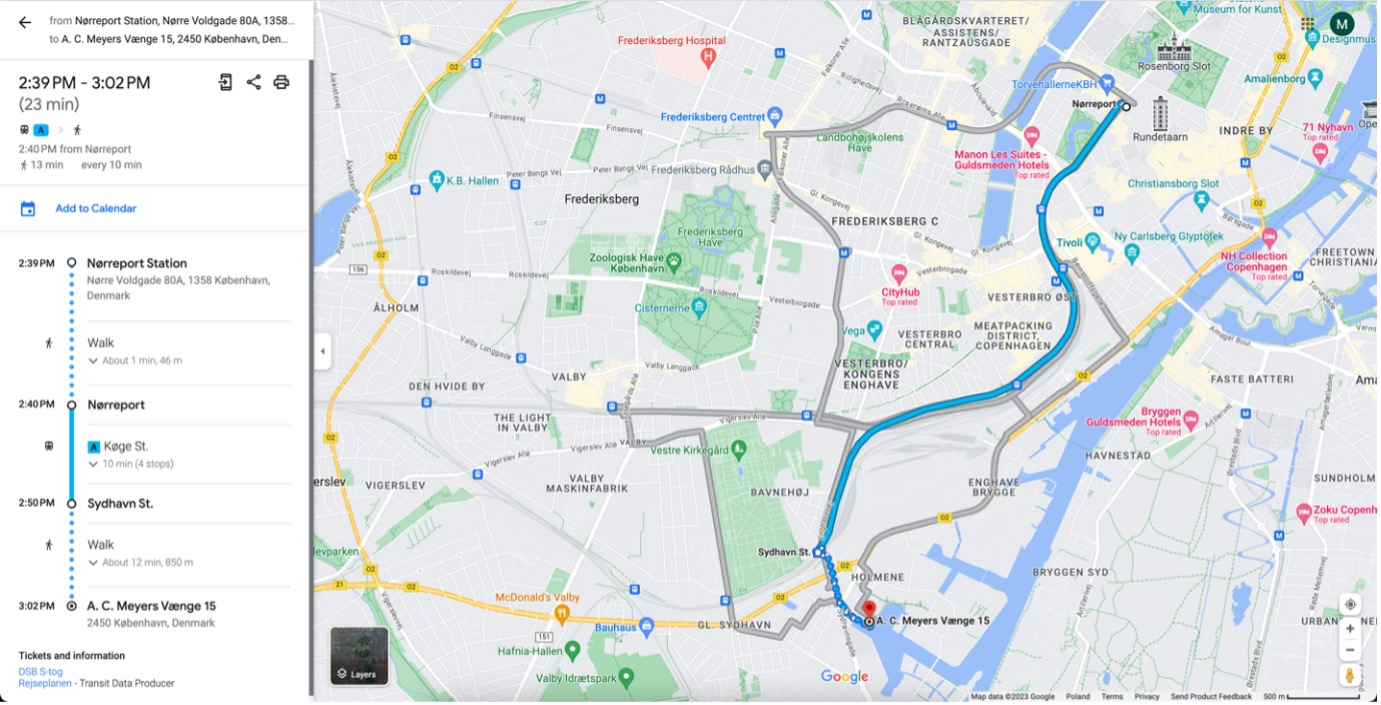
\includegraphics[width=\textwidth]{google-maps}
    \caption{Google Maps web UI.}
    \label{fig:figure6}
\end{figure}

Google Maps is another online service used for travelling.
It is one of the most extensive and detailed mapping databases globally.
Its comprehensive coverage includes even remote areas, making it a go to for travelers and commuters.
Whether you're navigating in unknown areas or exploring remote landmarks, Google Maps is sure to provide accurate
mapping data~\cite{googlemaps2023}.

\subsubsection{Usage}\label{subsubsec:usage}

The above-mentioned application is a widely used travel and commuting planner that provides detailed navigation and
route information and can also be seen in Figure~\ref{fig:figure6}.
While it offers estimated travel time and distance, it lacks a direct and user-friendly way to determine the cost of the
trip or the \unit{CO_{2}} footprint.
Users cannot easily access information about how much money the trip will cost, as Google Maps does not integrate with
financial or payment apps to calculate expenses like tolls, fuel, or public transportation fees.
This makes sense since Google tries to target a large international audience with the application, making is difficult
or nearly impossible to cover every localized payment solution or traveling restriction.
Similarly, it does not provide real-time data on the \unit{CO_{2}} emissions associated with the chosen route, making it
challenging for users to make informed decisions about their environmental impact.

\begin{wrapfigure}{l}{0.5\textwidth}
    \begin{center}
        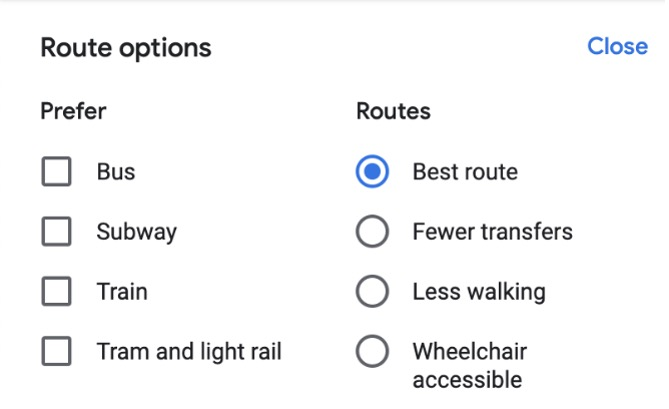
\includegraphics[width=0.4\textwidth]{google-maps-options}
    \end{center}
    \caption{Google Maps web UI options.}
    \label{fig:figure7}
\end{wrapfigure}

Users have very limited control over how cost and environmental factors are weighed in route calculations, as Google
Maps primarily focuses on travel time and distance.
The only available selection options, as can be seen in Figure~\ref{fig:figure7}, are preferences for means of
transportation and whether the route should be calculated with ``fewer transfers'', ``less walking'' or ``wheelchair
accessible'', where all three of the options seem to be tailored towards people with restricted mobility.

% textidote: ignore begin
\subsubsection{Ongoing developments}\label{subsec:ongoing-developments}
% textidote: ignore end

Google Maps continues to evolve with regular updates and new features.
Recent advancements include enhanced AR (Augmented Reality) navigation, which overlays digital information onto
a real-world environment through the user's smartphone camera.
With Augmented Reality navigation you would be able to see the navigation through your smartphone when holding it
vertically. \cite{googlemapsAR2023}
